%!TEX program = xelatex
\documentclass[cn,hazy,blue,14pt,通用]{elegantnote}
% \definecolor{geyecolor}{RGB}{199,237,204}
% \pagecolor{geyecolor}

\title{Git 学习笔记}
\author{Piex}
\institute{UCAS}

\version{1.0}
\date{\zhtoday}

\usepackage{array}

\begin{document}
\maketitle  %显示标题等信息
\centerline{
    
\includegraphics[width=0.2\textwidth]{git.jpg}
}
\newpage
\section{分区}
    \subsection{三大分区}
    \begin{itemize}
        \item 工作区:直接编辑的区域,对于新增的文件,如果没有add加入暂存区,就会以\textcolor{red}{红色(untracked/modified)}的形式放置在工作区.
        
        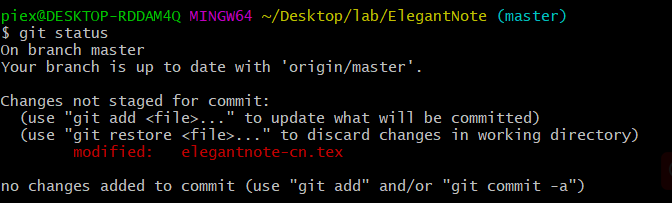
\includegraphics[width=0.8\textwidth]{workspace.jpg}
        \item 暂存区:数据暂时存放的区域(进入版本库之前),存放在.git/index目录下,Untracked files的文件,无法使用git commit –am 命令将文件添加到本地仓库中。git ls-files可以查看暂存区文件,要查看文件具体内容,需要使用git ls-files -s -- filename获得文件对应的blob对象,然后使用git cat-file -p [bolb的hash值前4位即可]查询内容。
        
        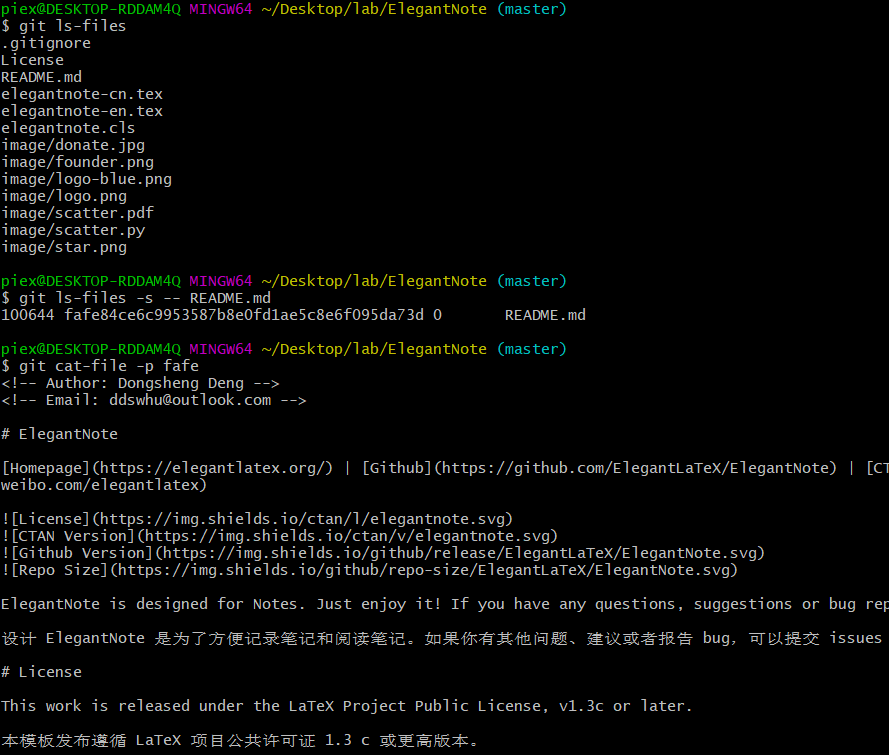
\includegraphics[width=0.8\textwidth]{cat-file.jpg}
        \item 版本库(本地仓库):暂存区commit的代码会放入版本库中,存放在.git目录下,push的时候版本库的数据全部发送到远程仓库中。
    \end{itemize}
    \subsection{涉及指令}
        \subsubsection{分区转换指令}
        \begin{itemize}
            \item git add:工作区->暂存区
            \item git commit:暂存区->版本库
            \item git push:版本库->远程仓库
        \end{itemize}
        \subsubsection{分区对比指令}
        \begin{itemize}
            \item git diff:工作区与暂存区对比
            
            git diff输出结果分析:---代表源文件,+++代表目标文件(通常工作区的文件被当做目标文件),空格开头的行是源文件和目标文件中都出现的行,-开头的行是只在源文件中出现的,+开头的行是只在目标文件中出现的,差异按照差异小结进行总结,每个差异小结的第一行都是定位语句,以@@开始,@@结束。如下图所示,@@ -1,7 +1,7 @@表示源文件第1行开始的7行和目标文件第1行开始的7行构成一个差异小结,差异内容是两行前面添加了\%和一个空格。


            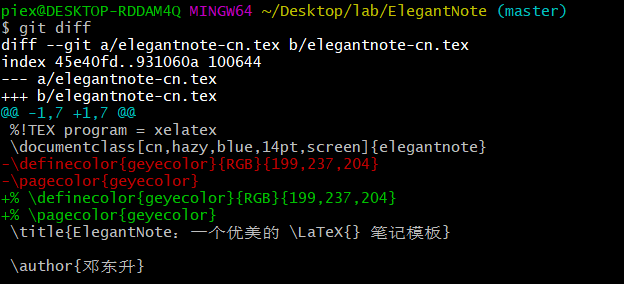
\includegraphics[width=0.8\textwidth]{diff.jpg}


            \item git diff head:工作区与版本库对比
            \item git diff -\space-cached:暂存区与版本库对比
        \end{itemize}
\section{原理}
    \subsection{git如何存储文件/目录信息}
        git init:初始化一个新的git项目,会在项目的根目录下创建.git的隐藏目录,其中.git目录下的objects目录,是存储文件变化的核心。objects下存放的文件名是哈希的“指纹”,文件内容就是git将信息压缩后形成的二进制文件。
    \subsection{git object的类型}
        三种:blob, tree, commit.

        文件存储为blob类型,文件夹为tree类型,每次提交的节点被存储为commit类型。\textcolor{red}{比较复杂,后面可以继续研究.}尝试对同一个文件的2行增加/减少注释多次并加入暂存区,发现objects下只有2个blob组件,查询后得知内容相同时便不会增加blob组件,因此2个blob组件分别对应注释前和注释后的暂存区文件。
\section{git分支}
    \subsection{git的目录树}
        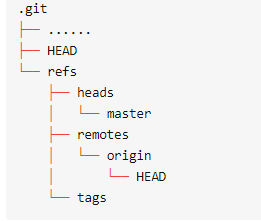
\includegraphics[width=0.5\textwidth]{git-tree.jpg}

        refs目录就是用来记录当前对分支的引用信息,包括本地分支,远程分支,标签。

        heads记录的是本地所有分支,remotes和\lstinline{\remotes\origin\HEAD}一样,指向对应的某个远程分支。\lstinline{heads\master}内容是“commit节点的hash值”,HEAD内容是“当前在哪个本地分支”,可以用git branch来创建其他分支,git chechkout来切换到其他分支,git branch -vv来查看分支信息。分支当前的指针指向最近一次commit的节点,通过谁创建的分支,就沿用谁的指针。(未被放入版本库的文件会在分支切换时被抛弃,造成严重后果)
    \subsection{分支的合并}
        merge和rebase两种 
        \begin{itemize}
            \item 相同点:都是从一个分支获取并合并到当前分支。
            \item 不同点:merge自动创建一个新的commit,如果遇到冲突,仅需要修改后重新commit,每次都记录了详细的commit,在commit频繁的时候会看到分支比较乱;
                         rebase是找公共的节点,直接合并之前commit历史,这样会是的分支发展历史比较简洁,去掉了merge commit,但是如果合并时出现了问题,没有留下痕迹不好定位。

                        git rebase -\space-abort:遇到冲突时放弃合并,回到rebase之前的状态;

                        git rebase -\space-continue:合并冲突,结合"git add 文件"命令一起,一步一步解决冲突;

                        git rebase -\space-skip:将引起冲突的commits丢弃掉.(最好不要在公共分支上使用rebase)
        \end{itemize}
            
            
    \subsection{分支的冲突}
        冲突的产生:冲突是从合并的时候产生的,git分支的合并,其实就是tree的合并,在feature/dev上执行git merge master时,git会先找到这两个分支(feature/1 \& feature/2)是从哪个指针创建出来的,称之为"merge base",然后检查这两次的tree是否一致,如果不一致说明一定有文件发生了修改。

        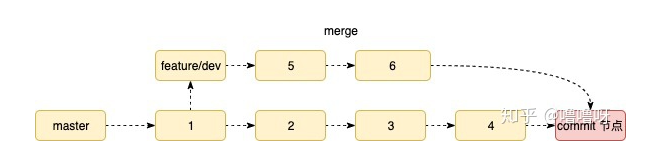
\includegraphics[width=0.8\textwidth]{merge.jpg}

        对于一个文件来说,有三种可能的情况:
        \begin{itemize}
            \item 文件在节点6,节点3以及merge base的hash值都相同,说明文件没有被修改过,不会有冲突;
            \item 文件在节点6和merge base(在节点3和merge base)的hash值相同,说明节点3(节点6)上的文件发生了修改,直接更新文件的变化即可;
            \item 文件在节点6、节点3以及merge bash上的hash值均不相同,冲突就产生了,也就是说节点6和节点3的文件都发生了修改,不知道哪个是最新的修改。
        \end{itemize}
\section{版本的回滚}
    \subsection{revert}
        执行git revert后,将回退到上一个commit的版本;
    \subsection{reset}
        git reset分为三种模式:soft,mixed,hard。由于每一次的commit都会产生与之对应的hash值,所以借助这个进行重置。

        \begin{itemize}
            \item git reset --hard commit.hash:会重置暂存区和工作区,完全重置为指定的commit节点,当前分支没有commit的代码会被清除;
            \item git reset --soft commit.hash:会保留工作目录,并把指定的commit节点与当前分支的差异都存入暂存区,即没有被commit的代码也会被保留下来;
            \item git reset commit.hash:不带参数即mixed模式,会保留工作目录,并把工作区,暂存区以及reset的差异都放到工作区,然后清除暂存区。因此执行后只要有所差异,文件都会变为红色,难以区分。
        \end{itemize}
        一般情况下,使用soft模式,既能保留暂存区,又能reset到某个分支。
\section{代码暂存}
    在当前分支工作时不得已需要切换到其他分支处理事情而不想commit时(commit多了会污染log),可以使用git stash将那些数据都暂存到git提供的栈中。
    \begin{itemize}
        \item git stash:暂存修改过的代码,保存到git栈中,然后将工作区还原成上一次commit的内容;
        \item git stash list:显示之前压栈的所有记录;
        \item git stash clear:清空git栈;
        \item git stash apply:从git栈中读取上一次暂存的那些代码,恢复工作区。
    \end{itemize}
\end{document}